\section{Experimental Setup and Main Results}
\label{sec:setup}

\subsection{Setup}

\paragraph{Benchmark.}
We use the cleaned release of LongMemEval-S~\citep{wu2025longmemeval}. The held-out set has \nm{datasets/heldout138/total} questions: every knowledge-update (KU, \nm{datasets/heldout138/KU}) and abstention (\nm{datasets/heldout138/Abs}) question outside the dev split, and \nm{datasets/heldout138/TR} temporal-reasoning questions. We split KU into \emph{KU-past} (\nm{datasets/heldout138/KU_past} questions whose wording asks about an earlier value, matched by a fixed list of cue words such as ``previously'' and ``before'') and \emph{KU-current} (\nm{datasets/heldout138/KU_current}). A disjoint dev split of the same question types was used only to calibrate $\tau$ and $\theta$ and to measure latency. For each question the stream ends right after the last evidence session; for KU questions this is the update, so at $\ell \geq 1$ the update is in flight. Abstention questions keep their full history. Unless stated otherwise, $p_\text{ooo}=0$.

\paragraph{Models.}
The extractor is glm-5.3-flash, run once per session. It sees user turns in full, assistant turns truncated to \nm{frozen_config/assistant_trunc_chars_extract} characters, and the list of keys already in use so that updates can reuse a key. Embeddings come from qwen3-embedding:0.6b, and $k=\nm{frozen_config/top_k_facts}$. The readers are gemma4 (12B, quantised, local), glm-5.3 and gpt-6-luna (API). All calls use temperature zero and seed \nm{stats/seed} and are cached, so each cell is a single deterministic run. Accuracy runs use the real broker (Redpanda, which speaks the Kafka protocol~\citep{kreps2011kafka}), Redis and PostgreSQL with pgvector; only timing is replaced by the barrier.

\paragraph{Judge and statistics.}
One judge, qwen3.8-flash, grades every answer in the paper with the per-type LongMemEval rubric, in the LLM-as-a-judge setup of \citet{zheng2023judging}. A second call labels abstention and, for KU questions, use of the superseded value, which gives the stale-read rate. Against qwen4-max on \nm{judge_agreement_qwen3.8-flash_vs_qwen4-max/n_pairs} verdict pairs from \nm{judge_agreement_qwen3.8-flash_vs_qwen4-max/n_questions} questions, Cohen's $\kappa$ is \nm{judge_agreement_qwen3.8-flash_vs_qwen4-max/correct/kappa} (\nm{judge_agreement_qwen3.8-flash_vs_qwen4-max/correct/kappa_ci95/0}--\nm{judge_agreement_qwen3.8-flash_vs_qwen4-max/correct/kappa_ci95/1}) for correctness and \nm{judge_agreement_qwen3.8-flash_vs_qwen4-max/stale_read/kappa} (\nm{judge_agreement_qwen3.8-flash_vs_qwen4-max/stale_read/kappa_ci95/0}--\nm{judge_agreement_qwen3.8-flash_vs_qwen4-max/stale_read/kappa_ci95/1}) for stale reads. Intervals are \nm{stats/ci_level_pct}\% percentile bootstrap intervals over questions (\nm{stats/bootstrap_resamples} resamples); pooled cells resample questions as clusters.

\subsection{Main results}
\label{sec:main}

% generated by scripts/build_paper_assets.py -- do not edit by hand
\begin{table*}[t]
\centering
\small
\setlength{\tabcolsep}{4pt}
\caption{LongMemEval-S held-out set (138 questions: 60 knowledge-update, 52 temporal, 26 abstention). Accuracy (\%) with 95\% bootstrap CIs over questions; stale-read = share of KU questions answered with the superseded value; tokens = mean reader prompt tokens. Async systems use the deterministic lag barrier with no reordering ($p_\text{ooo}=0$). Every cell is measured natively; the judge is qwen3.8-flash throughout.}
\label{tab:main138}
\begin{tabular}{lrcccccr}
\toprule
System & Lag & Overall & KU & Temporal & Abstention & Stale (\%) & Tokens \\
\midrule
\multicolumn{8}{l}{\textit{Reader: gemma4 (12B, local)}} \\
B1 sync (mutable) & 0 & 79.7\,{\scriptsize[72, 86]} & 83.3\,{\scriptsize[73, 92]} & 69.2\,{\scriptsize[56, 81]} & 92.3\,{\scriptsize[81, 100]} & 3.3 & 664 \\
B2 async & 1 & 23.2\,{\scriptsize[17, 30]} & 10.0\,{\scriptsize[3, 18]} & 3.8\,{\scriptsize[0, 10]} & 92.3\,{\scriptsize[81, 100]} & 68.3 & 656 \\
B3 recency (matched) & 1 & 58.0\,{\scriptsize[49, 66]} & 63.3\,{\scriptsize[52, 75]} & 32.7\,{\scriptsize[21, 46]} & 96.2\,{\scriptsize[88, 100]} & 30.0 & 1012 \\
Shadow v2 & 1 & 69.6\,{\scriptsize[62, 77]} & 80.0\,{\scriptsize[68, 90]} & 46.2\,{\scriptsize[33, 60]} & 92.3\,{\scriptsize[81, 100]} & 5.0 & 1204 \\
Lazy & 1 & 75.4\,{\scriptsize[68, 83]} & 76.7\,{\scriptsize[65, 87]} & 65.4\,{\scriptsize[52, 77]} & 92.3\,{\scriptsize[81, 100]} & 1.7 & 893 \\
DeltaWAL-Versioned & 0 & 83.3\,{\scriptsize[78, 89]} & 95.0\,{\scriptsize[88, 100]} & 65.4\,{\scriptsize[52, 77]} & 92.3\,{\scriptsize[81, 100]} & 1.7 & 791 \\
DeltaWAL-Versioned & 1 & 73.9\,{\scriptsize[67, 81]} & 88.3\,{\scriptsize[80, 95]} & 48.1\,{\scriptsize[35, 62]} & 92.3\,{\scriptsize[81, 100]} & 8.3 & 1255 \\
DeltaWAL-Versioned & 3 & 74.6\,{\scriptsize[67, 82]} & 88.3\,{\scriptsize[80, 95]} & 50.0\,{\scriptsize[37, 63]} & 92.3\,{\scriptsize[81, 100]} & 8.3 & 1266 \\
DeltaWAL-Versioned & 5 & 76.1\,{\scriptsize[69, 83]} & 91.7\,{\scriptsize[85, 98]} & 50.0\,{\scriptsize[37, 63]} & 92.3\,{\scriptsize[81, 100]} & 6.7 & 1288 \\
\midrule
\multicolumn{8}{l}{\textit{Reader: glm-5.3 (frontier, cloud)}} \\
B1 sync (mutable) & 0 & 81.9\,{\scriptsize[75, 88]} & 76.7\,{\scriptsize[65, 87]} & 82.7\,{\scriptsize[71, 92]} & 92.3\,{\scriptsize[81, 100]} & 0.0 & 664 \\
B2 async & 1 & 24.6\,{\scriptsize[17, 33]} & 11.7\,{\scriptsize[5, 20]} & 5.8\,{\scriptsize[0, 13]} & 92.3\,{\scriptsize[81, 100]} & 53.3 & 656 \\
B3 recency (matched) & 1 & 66.7\,{\scriptsize[59, 74]} & 80.0\,{\scriptsize[70, 90]} & 38.5\,{\scriptsize[25, 52]} & 92.3\,{\scriptsize[81, 100]} & 11.7 & 1012 \\
Shadow v2 & 1 & 84.8\,{\scriptsize[79, 91]} & 85.0\,{\scriptsize[75, 93]} & 80.8\,{\scriptsize[69, 90]} & 92.3\,{\scriptsize[81, 100]} & 0.0 & 1204 \\
Lazy & 1 & 82.6\,{\scriptsize[76, 88]} & 80.0\,{\scriptsize[68, 90]} & 80.8\,{\scriptsize[69, 92]} & 92.3\,{\scriptsize[81, 100]} & 0.0 & 893 \\
DeltaWAL-Versioned & 0 & 91.3\,{\scriptsize[86, 96]} & 96.7\,{\scriptsize[92, 100]} & 86.5\,{\scriptsize[77, 94]} & 88.5\,{\scriptsize[77, 100]} & 0.0 & 791 \\
DeltaWAL-Versioned & 1 & 91.3\,{\scriptsize[86, 96]} & 96.7\,{\scriptsize[92, 100]} & 86.5\,{\scriptsize[77, 94]} & 88.5\,{\scriptsize[77, 100]} & 0.0 & 1255 \\
DeltaWAL-Versioned & 3 & 91.3\,{\scriptsize[86, 96]} & 96.7\,{\scriptsize[92, 100]} & 86.5\,{\scriptsize[77, 94]} & 88.5\,{\scriptsize[77, 100]} & 0.0 & 1266 \\
\midrule
\multicolumn{8}{l}{\textit{Reader: gpt-6-luna (cloud)}} \\
B1 sync (mutable) & 0 & 81.2\,{\scriptsize[74, 88]} & 80.0\,{\scriptsize[70, 90]} & 78.8\,{\scriptsize[67, 88]} & 88.5\,{\scriptsize[77, 100]} & 3.3 & 664 \\
B2 async & 1 & 23.2\,{\scriptsize[16, 30]} & 11.7\,{\scriptsize[5, 20]} & 3.8\,{\scriptsize[0, 10]} & 88.5\,{\scriptsize[77, 100]} & 61.7 & 656 \\
B3 recency (matched) & 1 & 63.8\,{\scriptsize[56, 72]} & 71.7\,{\scriptsize[60, 82]} & 40.4\,{\scriptsize[27, 54]} & 92.3\,{\scriptsize[81, 100]} & 20.0 & 1012 \\
Shadow v2 & 1 & 81.9\,{\scriptsize[75, 88]} & 81.7\,{\scriptsize[72, 90]} & 76.9\,{\scriptsize[65, 88]} & 92.3\,{\scriptsize[81, 100]} & 1.7 & 1204 \\
Lazy & 1 & 79.0\,{\scriptsize[72, 86]} & 78.3\,{\scriptsize[67, 88]} & 73.1\,{\scriptsize[62, 85]} & 92.3\,{\scriptsize[81, 100]} & 0.0 & 893 \\
DeltaWAL-Versioned & 0 & 89.1\,{\scriptsize[84, 94]} & 93.3\,{\scriptsize[87, 98]} & 82.7\,{\scriptsize[73, 92]} & 92.3\,{\scriptsize[81, 100]} & 3.3 & 791 \\
DeltaWAL-Versioned & 1 & 88.4\,{\scriptsize[83, 93]} & 93.3\,{\scriptsize[87, 98]} & 80.8\,{\scriptsize[69, 90]} & 92.3\,{\scriptsize[81, 100]} & 3.3 & 1255 \\
DeltaWAL-Versioned & 3 & 88.4\,{\scriptsize[83, 93]} & 93.3\,{\scriptsize[87, 98]} & 80.8\,{\scriptsize[69, 90]} & 92.3\,{\scriptsize[81, 100]} & 3.3 & 1266 \\
\bottomrule
\end{tabular}
\end{table*}


\paragraph{Asynchrony without the WAL breaks updates.}
With one session in flight, B2 answers \nm{tab1/gemma4/B2_async/lag1/KU}--\nm{tab1/glm-5.3/B2_async/lag1/KU}\% of KU questions correctly across readers, against \nm{tab1/glm-5.3/B1_sync/lag0/KU}--\nm{tab1/gemma4/B1_sync/lag0/KU}\% for B1 (Table~\ref{tab:main138}); most errors are stale reads (\nm{tab1/glm-5.3/B2_async/lag1/stale_read_pct_KU}--\nm{tab1/gemma4/B2_async/lag1/stale_read_pct_KU}\% of KU answers), and temporal accuracy falls to at most \nm{tab1/glm-5.3/B2_async/lag1/temporal}\% because the last evidence session is the one in flight. A stronger reader does not help. B3's recency window recovers part of the loss (\nm{tab1/gemma4/B3_recency_matched_user/lag1/KU}--\nm{tab1/glm-5.3/B3_recency_matched_user/lag1/KU}\% on KU) but still reads stale values on \nm{tab1/glm-5.3/B3_recency_matched_user/lag1/stale_read_pct_KU}--\nm{tab1/gemma4/B3_recency_matched_user/lag1/stale_read_pct_KU}\% of KU questions: without epoch tags the reader sees a stale fact next to an undated raw turn and has no rule for choosing. B3's token budget was matched to an earlier measurement of DeltaWAL's prompt; in the final runs it averages \nm{tab1/gemma4/B3_recency_matched_user/lag1/mean_prompt_tokens} tokens against \nm{tab1/gemma4/deltawal_versioned/lag1/mean_prompt_tokens} for DeltaWAL-Versioned, so the match is approximate and favours DeltaWAL-Versioned.

\paragraph{DeltaWAL-Versioned removes most of the cost of asynchrony.}
The cleanest comparison is DeltaWAL-Versioned at lag $\ell$ against itself at $\ell=0$, where it reads the complete versioned store. For glm-5.3 the scores are identical at lags 0, 1 and 3 (\nm{tab1/glm-5.3/deltawal_versioned/lag1/overall}\% overall, \nmci{tab1/glm-5.3/deltawal_versioned/lag1/overall}); for gpt-6-luna, lags 1 and 3 give \nm{tab1/gpt-6-luna/deltawal_versioned/lag1/overall}\% against \nm{tab1/gpt-6-luna/deltawal_versioned/lag0/overall}\% at lag 0, with stale reads at \nm{tab1/glm-5.3/deltawal_versioned/lag1/stale_read_pct_KU}\% and \nm{tab1/gpt-6-luna/deltawal_versioned/lag1/stale_read_pct_KU}\%. Against B1, DeltaWAL-Versioned at lag 1 is higher on KU for all three readers, a gain Section~\ref{sec:history} traces to KU-past questions, and it acknowledges writes in milliseconds instead of seconds (Figure~\ref{fig:pareto}a). The WAL tail costs tokens: \nm{tab1/glm-5.3/deltawal_versioned/lag1/mean_prompt_tokens} prompt tokens at lag 1 against \nm{tab1/glm-5.3/deltawal_versioned/lag0/mean_prompt_tokens} at lag 0. Shadow and Lazy also beat B2 and B3 overall for every reader but stay below DeltaWAL-Versioned on KU (glm-5.3: \nm{tab1/glm-5.3/deltawal_shadow_v2/lag1/KU}\% and \nm{tab1/glm-5.3/deltawal_lazy/lag1/KU}\% against \nm{tab1/glm-5.3/deltawal_versioned/lag1/KU}\%); both drop stored facts that a newer item supersedes, the read-side erasure of Section~\ref{sec:history}.

\paragraph{The 12B reader loses temporal accuracy when the WAL tail is in the prompt.}
gemma4's temporal accuracy with DeltaWAL-Versioned drops from \nm{tab1/gemma4/deltawal_versioned/lag0/temporal}\% at lag 0 to \nm{tab1/gemma4/deltawal_versioned/lag1/temporal}\% (\nmci{tab1/gemma4/deltawal_versioned/lag1/temporal}) at lag 1 and stays there at lags 3 and 5, so its overall accuracy at lag 1 (\nm{tab1/gemma4/deltawal_versioned/lag1/overall}\%) is below B1's (\nm{tab1/gemma4/B1_sync/lag0/overall}\%), with overlapping intervals; glm-5.3 keeps \nm{tab1/glm-5.3/deltawal_versioned/lag1/temporal}\% on the same prompts (Figure~\ref{fig:pareto}b). In the \nm{forensics/q2_n} temporal questions gemma4 gets wrong under the DeltaWAL prompt at lag 1 but right under B1 or Lazy, it abstains or computes a date or count from the wrong item of a prompt that mixes facts and raw turns. Lazy, which turns the gated turns into facts first, keeps gemma4 at \nm{tab1/gemma4/deltawal_lazy/lag1/temporal}\% at the cost of an extraction call per query. A reader-capacity limit on long mixed prompts is a plausible cause; we did not isolate it.

\begin{figure*}[t]
\centering
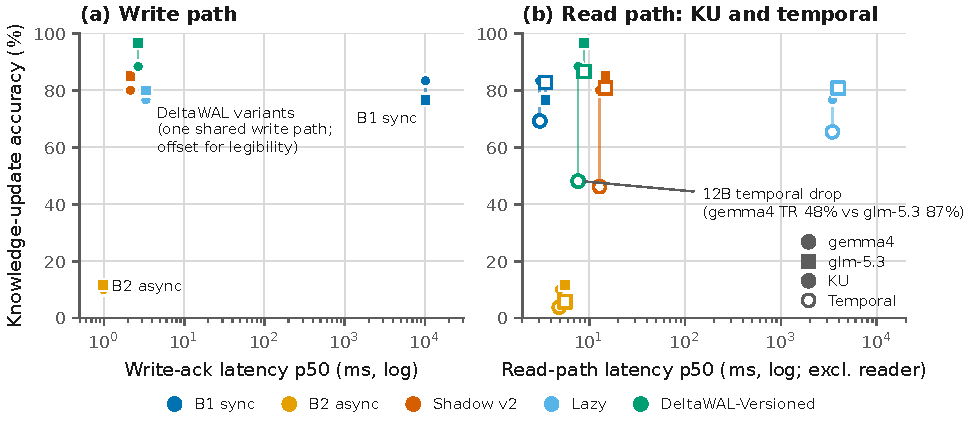
\includegraphics[width=\textwidth]{figures/fig2_pareto.pdf}
\caption{Accuracy against median latency for gemma4 (circles) and glm-5.3 (squares); async systems at lag 1, B1 at lag 0. (a) KU accuracy against write-acknowledgement latency: B1 waits for extraction (\nm{fig2/B1_sync/gemma4/write_ack_p50_ms}\,ms); all DeltaWAL variants share one write path (\nm{fig2/deltawal_versioned/gemma4/write_ack_p50_ms}\,ms; points offset for legibility). (b) KU (filled) and temporal (hollow) accuracy against read-path latency, excluding the reader. DeltaWAL-Versioned is plotted at the DeltaWAL read-path latency (\nm{fig2/deltawal_versioned/gemma4/read_p50_ms}\,ms), since it uses the same gate and merge. The annotation marks gemma4's temporal accuracy at lag 1 (\nm{fig2/deltawal_versioned/gemma4/temporal}\%) against glm-5.3's (\nm{fig2/deltawal_versioned/glm-5.3/temporal}\%). Latencies from Table~\ref{tab:latency}.}
\label{fig:pareto}
\end{figure*}
